%%%%%%%%%%%%%%%%%%%%%%% file template.tex %%%%%%%%%%%%%%%%%%%%%%%%%
%
% This is a general template file for the LaTeX package SVJour3
% for Springer journals.          Springer Heidelberg 2010/09/16
%
% Copy it to a new file with a new name and use it as the basis
% for your article. Delete % signs as needed.
%
% This template includes a few options for different layouts and
% content for various journals. Please consult a previous issue of
% your journal as needed.
%
%%%%%%%%%%%%%%%%%%%%%%%%%%%%%%%%%%%%%%%%%%%%%%%%%%%%%%%%%%%%%%%%%%%
%
% First comes an example EPS file -- just ignore it and
% proceed on the \documentclass line
% your LaTeX will extract the file if required
\begin{filecontents*}{example.eps}
%!PS-Adobe-3.0 EPSF-3.0
%%BoundingBox: 19 19 221 221
%%CreationDate: Mon Sep 29 1997
%%Creator: programmed by hand (JK)
%%EndComments
gsave
newpath
  20 20 moveto
  20 220 lineto
  220 220 lineto
  220 20 lineto
closepath
2 setlinewidth
gsave
  .4 setgray fill
grestore
stroke
grestore
\end{filecontents*}
%
\RequirePackage{fix-cm}
%
%\documentclass{svjour3}                     % onecolumn (standard format)
%\documentclass[smallcondensed]{svjour3}     % onecolumn (ditto)
\documentclass[smallextended]{svjour3}       % onecolumn (second format)
%\documentclass[twocolumn]{svjour3}          % twocolumn
%
\smartqed  % flush right qed marks, e.g. at end of proof
%
\usepackage{graphicx}
\usepackage{algpseudocode}
\usepackage{algorithm}
\usepackage{algorithmicx}
\usepackage{verbatim}
\usepackage{mathtools}
\usepackage{multirow}
\usepackage{colortbl}
\usepackage{balance}
\usepackage{hyperref}
\usepackage[table]{xcolor}
\usepackage{subcaption}

\usepackage{dirtree}

\usepackage{natbib}
\usepackage{amssymb}

\usepackage{tikz}
\usetikzlibrary{fit,automata,positioning}
\usetikzlibrary{decorations.pathmorphing}
\tikzset{snake it/.style={decorate, decoration=snake}}
\usepackage{booktabs} % For formal tables

\usepackage{kbordermatrix} % include package @ document preamble
%
% \usepackage{mathptmx}      % use Times fonts if available on your TeX system
%
% insert here the call for the packages your document requires
%\usepackage{latexsym}
% etc.
%
% please place your own definitions here and don't use \def but
% \newcommand{}{}
\renewcommand{\kbldelim}{(} % change default array delimiters to parentheses
\renewcommand{\kbrdelim}{)}

\newlength\Origarrayrulewidth

% horizontal rule equivalent to \cline but with 2pt width
\newcommand{\Cline}[1]{%
	\noalign{\global\setlength\Origarrayrulewidth{\arrayrulewidth}}%
	\noalign{\global\setlength\arrayrulewidth{3pt}}\cline{#1}%
	\noalign{\global\setlength\arrayrulewidth{\Origarrayrulewidth}}%
}

% draw a vertical rule of width 2pt on both sides of a cell
\newcommand\Thickvrule[1]{%
	\multicolumn{1}{!{\vrule width 2pt}c!{\vrule width 2pt}}{#1}%
}

% draw a vertical rule of width 2pt on the left side of a cell
\newcommand\Thickvrulel[1]{%
	\multicolumn{1}{!{\vrule width 2pt}c}{#1}%
}

% draw a vertical rule of width 2pt on the right side of a cell
\newcommand\Thickvruler[1]{%
	\multicolumn{1}{c!{\vrule width 2pt}}{#1}%
}

\newcommand\mc{\multicolumn{1}{c}{\cellcolor{lightgray}\textbf{1}}}
\newcommand{\term}[1]{\emph{#1}}
%
% Insert the name of "your journal" with
% \journalname{myjournal}
%
\begin{document}

\title{One Algorithm to Evaluate Them All: Unified Linear Algebra Based Approach to Evaluate Both Regular and Context-Free Path Queries%\thanks{Grants or other notes
%about the article that should go on the front page should be
%placed here. General acknowledgments should be placed at the end of the article.}
}
%\subtitle{Do you have a subtitle?\\ If so, write it here}

%\titlerunning{Short form of title}        % if too long for running head

\author{Ekaterina Shemetova  \thanks {The research was supported by the Russian Science Foundation, grant number: 18-11-00100}       \and
        Rustam Azimov \and
            Egor Orachev \and
             Ilya Epelbaum \and
             Semyon Grigorev
}

%\authorrunning{Short form of author list} % if too long for running head

\institute{E. Shemetova \at
              Saint Petersburg State University, 7/9 Universitetskaya nab., St. Petersburg, Russia\\
              Saint Petersburg Academic University, 8/3 Khlopin St., St. Petersburg, Russia\\
              JetBrains Research, Primorskiy prospekt 68-70, Building 1, St. Petersburg, Russia\\
              \email{katyacyfra@gmail.com}           %  \\
%             \emph{Present address:} of F. Author  %  if needed
           \and
R. Azimov \at
              Saint Petersburg State University, 7/9 Universitetskaya nab., St. Petersburg, Russia\\
              JetBrains Research, Primorskiy prospekt 68-70, Building 1, St. Petersburg, Russia\\
              \email{rustam.azimov19021995@gmail.com}           %  \\
%             \emph{Present address:} of F. Author  %  if needed
           \and
E. Orachev \at
              Saint Petersburg State University, 7/9 Universitetskaya nab., St. Petersburg, Russia\\
              JetBrains Research, Primorskiy prospekt 68-70, Building 1, St. Petersburg, Russia\\
              \email{egor.orachev@gmail.com}           %  \\
%             \emph{Present address:} of F. Author  %  if needed
           \and
I. Epelbaum \at
              Saint Petersburg State University, 7/9 Universitetskaya nab., St. Petersburg, Russia\\
              JetBrains Research, Primorskiy prospekt 68-70, Building 1, St. Petersburg, Russia\\
              \email{iliyepelbaun@gmail.com}           %  \\
%             \emph{Present address:} of F. Author  %  if needed
           \and
S. Grigorev \at
              Saint Petersburg State University, 7/9 Universitetskaya nab., St. Petersburg, Russia\\
              JetBrains Research, Primorskiy prospekt 68-70, Building 1, St. Petersburg, Russia\\
              \email{s.v.grigoriev@spbu.ru, semyon.grigorev@jetbrains.com}           %  \\
%             \emph{Present address:} of F. Author  %  if needed
           \and
}

\date{Received: date / Accepted: date}
% The correct dates will be entered by the editor


\maketitle

\begin{abstract}
Kronecker product based algorithm for context-free path querying (CFPQ) was proposed by \citet{10.1007/978-3-030-54832-2_6}. 
	We reduce this algorithm to operation over Boolean matrices and extend with mechanism to extract all paths of interest. 
	Also, we prove $O(n^3/\log{n})$ time complexity of the proposed algorithm, where $n$ is a number of vertices of the input graph. 
	Thus we provide an alternative way to construct a slightly subcubic algorithm for CFPQ which is based on linear algebra and on a classical graph-theoretic problem (incremental transitive closure), rather than the way proposed by~\cite{10.1145/1328438.1328460}. 
	Our evaluation shows that this algorithm is a good candidate to be a universal algorithm for both regular and context-free path querying. 
\keywords{Graph databases \and Regular path queries\and Context-free path queries \and CFL-reachability \and Recursive state machines \and Dynamic transitive closure}
% \PACS{PACS code1 \and PACS code2 \and more}
% \subclass{MSC code1 \and MSC code2 \and more}
\end{abstract}


\begin{acknowledgements}
We are grateful to Ekaterina Verbitskaia for careful reading and pointing out some mistakes.
\end{acknowledgements}
\section{Introduction}


Language-constrained path querying~\cite{barrett2000formal} is a technique for graph navigation querying.
This technique allows one to use formal languages as constraints on paths in edge-labeled graphs: path satisfies constraints if labels along it form a word from the specified language.

The utilization of regular languages as constraints, or \textit{Regular Path Querying} (RPQ), is most well-studied and widespread.
Different aspects of RPQs are actively studied in graph databases~\cite{10.1145/2463664.2465216, 10.1145/3104031,10.1145/2850413}, while regular constraints are supported in such popular query languages as PGQL~\cite{10.1145/2960414.2960421} and SPARQL\footnote{Specification of regular constraints in SPARQL property paths: \url{https://www.w3.org/TR/sparql11-property-paths/}. Access date: 07.07.2020.}~\cite{10.1007/978-3-319-25007-6_1} (property paths).
Nevertheless, there is certainly room for improvement of RPQ efficiency, and new solutions are being created~\cite{Wang2019,10.1145/2949689.2949711}.

At the same time, using more powerful languages, namely context-free languages, as constraints has gained popularity in the last few years.
\textit{Context-Free Path Querying} problem (CFPQ) was introduced by Mihalis Yannakakis in 1990 in~\cite{Yannakakis}.
Many algorithms were proposed since that time, but recently, Jochem Kuijpers et al. showed in~\cite{Kuijpers:2019:ESC:3335783.3335791} that state-of-the-art CFPQ algorithms are not performant enough for practical use.
This motivates us to develop new algorithms for CFPQ.

One promising way to achieve high-performance solutions for graph analysis problems is to reduce them to linear algebra operations.
This way, GraphBLAS~\cite{7761646} API, the description of basic linear algebra primitives, was proposed.
Solutions that use libraries that implement this API, such as SuiteSparce~\cite{10.1145/3322125} and CombBLAS~\cite{10.1177/1094342011403516}, show that reduction to linear algebra is a way to utilize high-performance parallel and distributed computations for graph analysis.

Rustam Azimov shows in~\cite{Azimov:2018:CPQ:3210259.3210264} how to reduce CFPQ to matrix multiplication.
Later, it was shown in~\cite{Mishin:2019:ECP:3327964.3328503} and~\cite{10.1145/3398682.3399163} that utilization of appropriate libraries for linear algebra for Azimov's algorithm implementation makes a practical solution for CFPQ.
However Azimov's algorithm requires transforming the input grammar to Chomsky Normal Form, which leads to the grammar size increase, and hence worsens performance, especially for regular queries and complex context-free queries.

To solve these problems, an algorithm based on automata intersection was proposed~\cite{10.1007/978-3-030-54832-2_6}.
This algorithm is based on linear algebra and does not require the transformation of the input grammar.
We improve the algorithm in this work.
We reduce the above mentioned solution to operations over Boolean matrices, thus simplifying its description and implementation.
Also, we show that this algorithm is performant enough for regular queries, so it is a good candidate for integration with real-world query languages: one algorithm can be used to evaluate both regular and context-free queries.

Moreover, we show that this algorithm opens the way to tackle a long-standing problem about the existence of truly-subcubic $O(n^{3-\epsilon})$ CFPQ algorithm ~\cite{10.1145/1328438.1328460, Yannakakis}.
Currently, the best result is an $O(n^3/\log{n})$ algorithm of Swarat Chaudhuri~\cite{10.1145/1328438.1328460}.
Also, there exist truly subcubic solutions which use fast matrix multiplication for some fixed subclasses of context-free languages~\cite{8249039}.
Unfortunately, this solutions cannot be generalized to arbitrary CFPQs.
In this work, we identify incremental transitive closure as a bottleneck on the way to achieve subcubic time complexity for CFPQ.

To sum up, we make the following contributions.
\begin{enumerate}
	\item We rethink and improve the CFPQ algorithm based on tensor-product proposed by Orachev et al. ~\cite{10.1007/978-3-030-54832-2_6}.
	We reduce this algorithm to operations over Boolean matrices.
	As a result, all-path query semantics is handled, as opposed to the previous matrix-based solution which handles only the single-path semantics.
	Also, both regular and context-free grammars can be used as queries.
	We prove the correctness and time complexity for the proposed algorithm.
	\item We demonstrate the interconnection between CFPQ and incremental transitive closure.
	We show that incremental transitive closure is a bottleneck on the way to achieve faster CFPQ algorithm for general case of arbitrary graphs as well as for special families of graphs, such as planar graphs.
	\item We implement the described algorithm and evaluate it on real-world data for both RPQ and CFPQ. Results show that the proposed solution is comparable with existing solutions for CFPQ and RPQ, thus it is a promising way to create a unified algorithm for both CFPQ and RPQ evaluation.
\end{enumerate}
\section{Preliminaries}
\label{sec:prel}
\label{preliminaries}
\paragraph{Formal languages.} 
A \textit{context-free grammar} is a 4-tuple $G = (\Sigma, N, P, S)$, where $\Sigma$ is a finite set of alphabet symbols,  $N$ is a set of nonterminal symbols, $P$ is a set of production rules and $S$ is a start nonterinal. $L(G)$ is a context-free language generated by context-free grammar $G$. We use the notation $A \stackrel {*}{\Rightarrow } w$  to denote that the string $w \in \Sigma^*$ can be derived from a nonterminal $A$ by sequence of applying the production rules from $P$. A \textit{parse tree} is an entity which represents the structure of the derivation of a terminal string from some nonterminal.


A grammar $G$ is said to be is in the \textit{Chomsky normal form}, if all production rules of $P$ are of the form:
$A \rightarrow BC$, $A \rightarrow a$ or $S \rightarrow \varepsilon$, where $A, B, C \in N$ and $a \in \Sigma$. 


The set of all context-free languages is identical to the set of languages accepted by pushdown automata (PDA). \textit{Pushdown automaton} is a 7-tuple $M = (Q, \Sigma, \Gamma, \delta, q_0, Z, F)$, where $Q$ is a finite set of states, $\Sigma$ is a input alphabet, $\Gamma$ is a finite set which is called the stack alphabet, $\delta$ is a finite subset of $Q \times (\Sigma \cap \{\varepsilon\}) \times \Gamma \times Q \times \Gamma^*$,
$q_{0}\in Q$ is the start state, $Z \in \Gamma$ is the initial stack symbol and
$F\subseteq Q$ is the set of accepting states.


A \textit{regular language} is a language that can be expressed with a regular expression or a deterministic or non-deterministic finite automata.
A \textit{nondeterministic finite automaton} (NFA) is represented by a 5-tuple, $(Q,\Sigma ,\delta ,Q_{0},F)$, where $Q$ is a finite set of states, $\Sigma$ is a finite set of input symbols, $\delta:Q\times \Sigma \rightarrow 2^{|Q|}$ is a transition function, $Q_0 \subseteq Q$ is a set of inial states, $F \subseteq Q$ is a set of accepting (final) states. \textit{Deterministic finite automaton} is a NFA with the following restrictions: each of its transitions is uniquely determined by its source state and input symbol, and reading an input symbol is required for each state transition.


 For a language $L$ over an alphabet $\Sigma$, its rational index $\rho_L$ is a function defined as follows:
$$\rho_L(n) = \max\{\min\{|w|:w \in L \cap K\}, K \in {Rat}_n, L \cap K \neq \emptyset\},$$ where $|w|$ is the length of a word $w$ and ${Rat}_n$ denotes the set of regular languages on an alphabet $\Sigma$, recognized by a finite nondeterministic automation with at most $n$ states.
\paragraph{Bounded-oscillation languages.} 
Oscillation is defined using a hierarchy of \textit{harmonics}. Let $\bar{a}$ be a \textit{push}-move and $a$ be a \textit{pop}-move. Then a PDA run $r$ can be described by a well-nested sequence $\alpha(r)$ of $\bar{a}$-s and $a$-s. Two positions $i<j$ form a \textit{matching pair} if the corresponding $\bar{a}$ at $i$-th position of the sequence matches with $a$ at $j$-th position. For example, word $\bar{a}\bar{a}\bar{a}aa\bar{a}aa$ has the following set of matching pairs: $\{(1, 8), (2, 5), (3, 4), (6, 7)\}$ ($\bar{a}(\bar{a}(\bar{a}a)a)(\bar{a}a)a$).


Harmonics are inductively defined as follows:
\begin{itemize}
\item  order 0 harmonic $h_0$ is $\varepsilon$
\item  $h_{(i+1)}$ harmonic is $\bar{a}h_ia\ \bar{a}h_ia$.
\end{itemize}
\begin{figure}
\centering
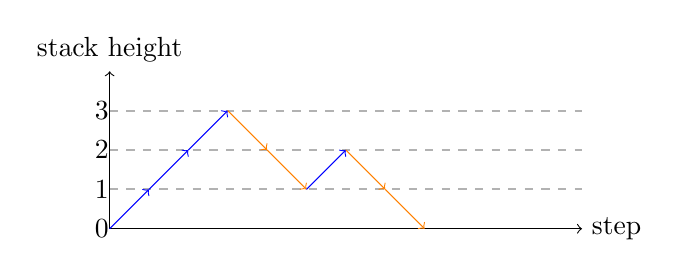
\begin{tikzpicture}
    \draw[thick, dashed, opacity=0.3] (0,0.5) -- (6,0.5);
     \draw[thick, dashed, opacity=0.3] (0,1) -- (6,1);
      \draw[thick, dashed, opacity=0.3] (0,1.5) -- (6,1.5);
      \draw[->] (0,0) -- (6,0) node[right] {step};
      \draw[->] (0,0) -- (0,2) node[above] {stack height};
     \draw[->, blue] (0,0) -- (0.5,0.5);
      \draw[->, blue] (0.5,0.5) -- (1,1);
      \draw[->, blue] (1,1) -- (1.5,1.5);
       \draw[->, orange] (1.5,1.5) -- (2,1);
    \draw[->, orange] (2,1) -- (2.5,0.5);
    \draw[->, blue] (2.5,0.5) -- (3,1);
    \draw[->, orange] (3,1) -- (3.5,0.5);
 \draw[->, orange] (3.5,0.5) -- (4,0);
\node (null) at (-0.1, 0) {0}; 
\node (one) at (-0.1, 0.5) {1}; 
\node (two) at (-0.1, 1) {2}; 
\node (three) at (-0.1, 1.5) {3}; 
    \end{tikzpicture}
\caption{Stack heights during the run of PDA.}
\label{oscb}
\end{figure}


PDA run $r$ is \textit{k-oscillating} if the harmonic of order $k$ is the greatest harmonic that occurs in $r$ after removing $0$ or more matching pairs. \textit{Bounded-oscillation languages} are languages accepted by pushdown automata with all runs $k$-oscillating. It is important that the problem whether a given CFL is a bounded-oscillation language is undecidable \cite{BoundOsc}.
\begin{example}
Consider Figure \ref{oscb}. It shows how the stack height changes during the run of a PDA. Corresponding well-nested word $\alpha(r)$ is $\bar{a}\bar{a}\bar{a}aa\bar{a}aa$. The greatest harmonic in this word is order 1 harmonic (moves forming harmonic are marked in bold, removed matching pairs are $(1, 8)$ and $(2, 5)$): $\bar{a}\bar{a}\mathbf{\bar{a}a}a\mathbf{\bar{a}a}a$, therefore oscillation of the run $r$ is 1.
\end{example}


The oscillation of a parse tree of a context-free grammar can be defined similiarly to the oscillation of a PDA run. Given a parse tree $t$, we define corresponding well-nested word $\alpha(t)$ inductively as follows:
\begin{itemize}
\item if $n$ is the root of $t$ then $\alpha(t) = \bar{a}\alpha(n)$
\item if $n$ is a leaf then $\alpha(n)=a$
\item if $n$ has $k$ children then $\alpha(n) = a\underbrace{\bar{a}...\bar{a}}_\text{$k$ times}\alpha(n_1)...\alpha(n_k)$
\end{itemize}


Moreover, given a PDA run $r$, there exists a corresponding parse tree $t$ with the same well-nested word $\alpha(t)=\alpha(r)$ and vice versa \cite{BoundOsc}.


The oscillation of a parse tree is closely related with its $dimension$. For each node $v$ in a tree $t$, its dimension $dim(v)$ is inductively defined as follows:
\begin{itemize}
\item if $v$ is a leaf, then $dim(v)$ = 0
\item if $v$ is an internal node with $k$ children $v_1, v_2, ..., v_k$ for $k \ge 1$, then 
$$
dim(v) = 
 \begin{cases}
   \max_{i \in \{1...k\}}dim(v_i) &\text{if there is a unique maximum}\\
   \max_{i \in \{1...k\}}dim(v_i)+1 &\text{otherwise}
 \end{cases}
$$
\end{itemize}


Dimension of a parse tree $t$ $dim(t)$ is a dimension of its root.  It is observable from the definition that dimension of a tree $t$ is the height of the largest perfect binary tree, which can be obtained from $t$ by contracting edges and accordingly identifying vertices. A tree with dimension $dim(t) = 2$ is illustrated in Figure \ref{oscbtree}.
\begin{figure}
\centering
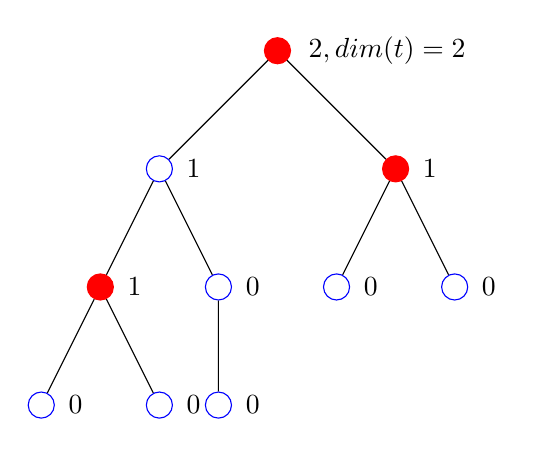
\begin{tikzpicture}[
level 1/.style={sibling distance=3cm},
level 2/.style={sibling distance=1.5cm}]
%\tikzstyle{every node}=[circle,draw]

\node[circle,draw] (Root) [ fill=red, red] {}
    child {
    node[circle,draw, blue] (l) {} 
    child { node[circle,draw, fill=red, red](ll) {}
            child { node[circle,draw, blue] (p) {} }
            child { node[circle,draw, blue] (pl) {} }
             }
    child { node[circle,draw, blue](lr) {} 
          child { node[circle,draw, blue] (plr) {} }
      }
}
child {
    node[circle,draw,  fill=red, red] (r) {}
    child { node[circle,draw, blue] (rl) {}} 
    child { node[circle,draw, blue] (rr) {} }
};
\node  [right=0.05cm of p] {0};
\node  [right=0.1cm of Root] {$2, dim(t)=2$};
\node  [right=0.05cm of l] {1};
\node  [right=0.05cm of r] {1};
\node  [right=0.05cm of ll] {1};
\node  [right=0.05cm of lr] {0};
\node  [right=0.05cm of pl] {0};
\node  [right=0.05cm of plr] {0};
\node  [right=0.05cm of rl] {0};
\node  [right=0.05cm of rr] {0};
\end{tikzpicture}
\caption{A tree $t$ with $dim(t)=2$. Nodes having children without unique maximum are filled.}
\label{oscbtree}            
\end{figure}


It is known that the dimension of parse trees and its oscillation are in linear relationship.

\begin{lemma}[\cite{BoundOsc}]
\label{boscdim}
Let a grammar $G = (\Sigma, N, P, S)$ be in Chomsky normal form and let $t$ be a parse tree of $G$. Then $osc(t) - 1 \le dim(t) \le 2osc(t)$.
\end{lemma}
\paragraph{Context-free language reachability.} 
A \textit{directed labeled graph} is a triple $D = (Q, \Sigma, \delta)$, where $Q$ is a finite set of nodes, $\Sigma$ is a finite set of alphabet symbols,
and $\delta \subseteq Q \times \Sigma \times Q$ is a finite set of labeled edges. Let $L(D)$ denote a graph language~--- a regular language, which is recognized by the NFA $(Q,\Sigma ,\delta ,Q, Q)$ obtained from $D$ by setting every state as inial and accepting.


Let $i\pi j$ denote a unique path between nodes $i$ and $j$ of the input graph and $l(\pi)$ denote a unique string obtained by concatenating edge labels along the path $\pi$. Then the CFL-reachability can be defined as follows.
\begin{definition}[Context-free language reachability]
Let $L \subseteq \Sigma^*$ be a context-free language and $D = (Q, \Sigma, \delta)$ be a directed labeled graph. Given two nodes $i$ and $j$ we say that $j$ is \textit{reachable} from $i$ if there exists a path $i \pi j$, such that $l(\pi) \in L$. 
\end{definition}
There are four varieties of CFL-reachability problems: all-pairs problem, single-source problem, single-target problem and single-source/single-target problem \cite{RepsBasic}. In this paper we consider all-pairs problem. The \textit{all-pairs problem} is to determine all pairs of nodes $i$ and $j$ such that $j$ is reachable from $i$. 




\section{Context-free path querying by Kronecker product}


In this section we introduce the algorithm for CFPQ which is based on Kronecker product of Boolean matrices.
The algorithm solves all-pairs CFPQ in all-path semantics (according to~\cite{hellingsPathQuerying}) and works in two steps.
\begin{enumerate}
\item \emph{Index creation}.
 In this step, the algorithm computes an index which contains information necessary to restore paths for given pairs of vertices.
 This index can be used to solve the reachability problem without extracting paths.
 Note that this index is finite even if the set of paths is infinite.
\item \emph{Paths extraction}.
All paths for the given pair of vertices can be enumerated by using the index.
Since the set of paths can be infinite, all paths cannot be enumerated explicitly, and advanced techniques such as lazy evaluation are required for the implementation.
Nevertheless, a single path can always be extracted with standard techniques.
\end{enumerate}

In the following subsections we describe these steps, prove correctness of the algorithm, and provide time complexity estimations.
For the first step we firstly introduce na{\"i}ve algortihm. After that we show how to achieve cubic time complexity by using dynamic transitive closure algorithm and shave off a logarithmic factor to achive the best known time complexity for CFPQ.

After that we provide step-by-step example of query evaluation by using the proposed algorithm.

\subsection{Index Creation Algorithm}

The \textit{index creation} algorithm outputs the final adjacency matrix for the input graph with all pairs of vertices which are reachable through some nonterminal in the input grammar $G$, as well as the index matrix, which is to be used to extract paths in the \textit{path extraction} algorithm.

The algorithm is based on the generalization of the FSM intersection for an RSM,  and the edge-labeled directed input graph.
Since the RSM is composed as a set of FSMs, it could be easily presented as an adjacency matrix for some graph over labels set .
As shown in the Def.~\ref{def:bool:product}, we can apply Kronecker product from Boolean matrices to \textit{intersect} the RSM and the input graph to some extent.
But the RSM contains the nonterminal symbols with additional \textit{recursive calls} logic, which requires \textit{transitive closure} step to extract such symbols.

The core idea of the algorithm comes from Kronecker product and transitive closure.
The algorithm boils down to the iterative Kronecker product evaluation for the RSM $R$ adjacency matrix $\mathcal{M}_1$ and the input graph $\mathcal{G}$ adjacency matrix $\mathcal{M}_2$, followed by transitive closure, extraction of nonterminals and updating the graph adjacency matrix $\mathcal{M}_2$.
Listing~\ref{tensor:cfpq:cubic} shows main steps of the algorithm.
\begin{algorithm}[h]
\floatname{algorithm}{Listing}
\begin{algorithmic}[1]
\footnotesize
\caption{Kronecker product based CFPQ using dynamic transitive closure}
\label{tensor:cfpq:cubic}
\Function{contextFreePathQuerying}{G, $\mathcal{G}$}
    % Input data preparation
   \State{$n \gets$ The number of nodes in $\mathcal{G}$}
    \State{$R \gets$ Recursive automata for $G$}
    \State{$\mathcal{M}_1 \gets$ Boolean adjacency matrix for $R$}
    \State{$\mathcal{M}_2, \mathcal{A}_2 \gets$ Boolean adjacency matrix for $\mathcal{G}$}
    %\State{$M_3 \gets$ The empty matrix}
    \State{$C_3 \gets$ The empty matrix of size $|R|n \times |R|n$}
    % Eps-transition handling for graph
    \For{$s \in 0..dim(\mathcal{M}_1)-1$}
        \For{$S \in \textit{getNonterminals}(R,s,s)$}
            \For{$i \in 0..dim(\mathcal{M}_2)-1$}
                \State{$M^S_2[i,i] \gets 1 $}
            \EndFor
        \EndFor
    \EndFor
    \While{$\mathcal{M}_2$ is changing}
        \State{$M_3' \gets \bigvee_{M^S \in \mathcal{M}_1 \otimes \mathcal{A}_2} M^S$}
        %\State{$\mathcal{A}_2 \gets$ The empty matrix of size $n \times n$}
        \State{$\mathcal{A}_2 \gets$ The empty matrix}
        \State{$C_3' \gets$ The empty matrix of size $|R|n \times |R|n$}
        %\Comment{Evaluate Kroncker product}
        \For{$(i,j) \mid M_3'[i,j] \neq 0$}
            %\State{$C_3'[i,j] \gets 1$}
            \State{$C_3' \gets \textit{add}(C_3, C_3', i, j)$}
            \Comment{Updating the transitive closure}
            \State{$C_3 \gets C_3 + C_3'$}
        \EndFor
        %\State{$n \gets$ dim($M_3)$}
        %\Comment{Matrix $M_3$ size = $n \times n$}
        % Add non-terminals (possibly new)
        \For{$(i,j)\ |\ C_3'[i,j] \neq 0$}
                \State{$s, f \gets \textit{getStates}(C_3',i,j)$}
                \State{$x, y \gets \textit{getCoordinates}(C_3',i,j)$}
                \For{$S \in \textit{getNonterminals}(R,s,f)$}
                    \State{$M^S_2[x,y] \gets 1$}
                    \State{$A^S_2[x,y] \gets 1$}
                \EndFor
        \EndFor
    \EndWhile
\State \Return $\mathcal{M}_2, C_3$
\EndFunction
% \Function{add}{$C, C', i, j$}
%     \State{$C'[i,j] \gets {1}$}
%     \For{$(u,v) \mid C[u,i] = C[j,v] = 1, C[u,j] = C[u,v] = 0$}
%         \State{$C'[u,v] \gets {1}$}
%     \EndFor
%     \State \Return{$C'$}
% \EndFunction
\Function{getStates}{$C, i, j$}
    \State{$r \gets dim(\mathcal{M}_1)$}
    \Comment{$\mathcal{M}_1$ is adjacency matrix for $R$}
    \State \Return{$\left\lfloor{i / r}\right\rfloor, \left\lfloor{j / r}\right\rfloor$}
\EndFunction
\Function{getCoordinates}{$C, i, j$}
    \State{$n \gets dim(\mathcal{M}_2)$}
    \Comment{$\mathcal{M}_2$ is adjacency matrix for $\mathcal{G}$}
    \State \Return{$i \bmod n, j \bmod n$}
\EndFunction
\end{algorithmic}
\end{algorithm}
\subsubsection{Application of Dynamic Transitive Closure}
It is easy to see that the most time-consuming steps of the algorithm are the Kronecker product and transitive closure computations.
Note that the adjacency matrix $\mathcal{M}_2$ is always changed incrementally i. e. elements (edges) are added to $\mathcal{M}_2$ (and are never deleted from it) at each iteration of the algorithm.
So it is not necessary to recompute the whole product or transitive closure if an appropriate data structure is maintained.

To compute the Kronecker product, we employ the fact that it is left-distributive.
Let $\mathcal{A}_2$ be a matrix with newly added elements and $\mathcal{B}_2$ be a matrix with the all previously found elements, such that $\mathcal{M}_2 = \mathcal{A}_2 + \mathcal{B}_2$.
Then by the left-distributivity of the Kronecker product we have $\mathcal{M}_1 \otimes \mathcal{M}_2 = \mathcal{M}_1 \otimes (\mathcal{A}_2 + \mathcal{B}_2) = \mathcal{M}_1\otimes \mathcal{A}_2 + \mathcal{M}_1 \otimes \mathcal{B}_2$.
Note that $\mathcal{M}_1 \otimes \mathcal{B}_2$ is known and is already in the matrix $\mathcal{M}_3$ and its transitive closure also is already in the matrix $C_3$, because it has been calculated at the previous iterations, so it is left to update some elements of $\mathcal{M}_3$ by computing $\mathcal{M}_1\otimes \mathcal{A}_2$.


The fast computation of transitive closure can be obtained by using incremental dynamic transitive closure technique. Now we describe the function $add$ from Listing \ref{tensor:cfpq:cubic}. Let $C_3$ be a transitive closure matrix of the graph $G$ with $n$ vertices. We use an approach by~\cite{IBARAKI198395} to maintain dynamic transitive closure. The key idea of their algorithm is to recalculate reachability information only for those vertices, which become reachable after insertion of the certain edge. We have modified it to achieve a logarithmic speed-up.


For each newly inserted edge $(i, j)$ and every node $u \neq j$ of $G$ such that $C_3[u, i] = 1$ and $C_3[u, j]=0$, one needs to perform operation $C_3[u,v] = C_3[u, v] \wedge C_3[j, v]$ for every node $v$, where $1 \wedge 1 = 0 \wedge 0 = 1 \wedge 0 = 0$ and $0 \wedge 1 = 1$.
Notice that these operations are equivalent to the element-wise (Hadamard) product of two vectors of size $n$, where multiplication operation is denoted as $\wedge$. To check whether $C_3[u, i] = 1$ and $C_3[u, j]=0$ one needs to multiply two vectors: the first vector represents reachability of the given vertex $i$ from other vertices $\{u_1, u_2, ..., u_n\}$ of the graph and the second vector represents the same for the given vertex $j$. The operation $C_3[u, v] \wedge C_3[j, v]$ also can be reduced to the computation of the Hadamard product of two vectors of size $n$ for the given $u_k$. The first vector contains the information whether vertices  $\{v_1, v_2, ..., v_n\}$ of the graph are reachable from the given vertex $u_k$ and the second vector represents the same for the given vertex $j$. The element-wise product of two vectors can be calculated naively in time $O(n)$. Thus, the time complexity of the transitive closure can be reduced by speeding up element-wise product of two vectors of size $n$.


To achieve logarithmic speed-up, we use the Four Russians' trick.
First we split each vector into $n/\log n$ parts of size $\log n$.
Then we create a table $T$ such that $T(a, b)$ = $a \wedge b$ where $a, b \ \in {\{0,1\}}^{\log n}$.
This takes time $O(n^2 \log n)$, since there are $2^{\log n} = n$ variants of Boolean vectors of size $\log n$ and hence $n^2$ possible pairs of vectors $(a, b)$ in total, and each component takes $O(\log n)$ time.
With table $T$, we can calculate product of two parts of size $\log n$ in constant time.
There are $n/\log n$ such parts, so the element-wise product of two vectors of size $n$ can be calculated in time $O(n/\log n)$ with $O(n^2 \log n)$ preprocessing.

\begin{theorem}
    Let $\mathcal{G} =  \langle V,E,L\rangle$ be a graph and $G = \langle\Sigma, N, S, P\rangle$ be a grammar.
    Let $\mathcal{M}_{2}$ be a resulting adjacency matrix after the execution of the algorithm in Listing~\ref{tensor:cfpq:cubic}. Then for any valid indices $i, j$ and for each nonterminal $N_i \in N$ the following statement holds: the cell $M_{2,(k)}^{N_i}[i,j]$ contains $\{1\}$, iff there is a path $i\pi j$ in the graph $\mathcal{G}$ such that $ N_i \xrightarrow{*} l(\pi)$.
\end{theorem}{}
\begin{proof}
    The main idea of the proof is to use induction on the height of the derivation tree obtained on each iteration.
\end{proof}{}

\begin{theorem}{}
\label{theorem: subcubic}
    Let $\mathcal{G} = \langle V,E,L \rangle$ be a graph and $G = \langle\Sigma, N, S, P\rangle$ be a grammar.
    The algorithm from Listing~\ref{tensor:cfpq:cubic} calculates resulting matrices $\mathcal{M}_2$ and $C_3$ in $O({|P|}^3n^3/\log (|P|n))$ time where $n = |V|$. Moreover, the maintaining of the dynamic transitive closure dominates the cost of the algorithm.
\end{theorem}

\begin{proof}
 Let $|\mathcal{A}|$ be a number of non-zero elements in a matrix $\mathcal{A}$. Consider the total time which is needed for computing the Kronecker products. The elements of the matrices $\mathcal{A}_2^{(i)}$ are pairwise distinct on every $i$-th iteration of the algorithm therefore the total number of operations is $\sum\limits_i{T(\mathcal{M}_1 \otimes \mathcal{A}_2^{(i)})} = |\mathcal{M}_1| \sum\limits_i {|\mathcal{A}_2^{(i)}|} = (|N| + |\Sigma|){|P|}^2 \sum\limits_i {|\mathcal{A}_2^{(i)}|} = O({(|N| + |\Sigma|)}^2{|P|}^2 n^2).$


Now we derive the time complexity of maintaining the dynamic transitive closure.
Notice that $C_3$ has size of the Kronecker product of $\mathcal{M}_1 \otimes \mathcal{M}_2$, which is equal to $|R|n \times |R|n = |P|n \times |P|n$ so no more than ${|P|}^2n^2$ edges will be added during all iterations of the Algorithm.
Checking condition whether $C_3[u, i] = 1$ and $C_3[u, j]=0$ for every node $u \in V$ for each newly inserted edge $(i, j)$ requires one multiplication of vectors per insertion, thus total time is $O({|P|}^3n^3/\log (|P|n))$.
Note that after checking the condition, at least one element $C[u', j]$ changes value from 0 to 1 and then never becomes 0 for some $u'$ and $j$.
Therefore the operation $C_3[u',v] = C_3[u', v] \wedge C_3[j, v]$ for all $v \in V$ is executed at most once for every pair of vertices $(u',j)$ during the entire computation implying that the total time is equal to $O({|P|}^2n^2|P|n/\log (|P|n))=O({|P|}^3n^3/\log (|P|n))$ (using the  multiplication of vectors).


The matrix $C_3'$ contains only new elements, therefore $C_3$ can be updated directly using only $|C_3'|$ operations and hence ${|P|}^2n^2$ operations in total.
The same holds for cycle in line 17 of the algorithm from Listing~\ref{tensor:cfpq:cubic}, because operations are performed only for non-zero elements of the matrix $|C_3'|$.
Finally, the time complexity of the algorithm is $O({(|N| + |\Sigma|)}^2{|P|}^2 n^2) + O({|P|}^2n^2) + O({|P|}^2n^2 \log (|P|n)) + O({|P|}^3n^3/\log (|P|n)) + O({|P|}^2n^2)= O({|P|}^3n^3/\log (|P|n))$. \qed
\end{proof}

The complexity analysis of the Algorithm~\ref{tensor:cfpq:cubic} shows that the maintaining of the incremental transitive closure dominates the cost of the algorithm. Thus, CFPQ can be solved in truly subcubic $O(n^{3-\varepsilon})$ time if there is an incremental dynamic algorithm for the transitive closure for a graph with $n$ vertices with preprocessing time $O(n^{3-\varepsilon})$ and total update time $O(n^{3-\varepsilon})$. Unfortunately, such an algorithm is unlikely to exist: it was proven that there is no incremental dynamic transitive closure algorithm for a graph with $n$ vertices and at most $m$ edges with preprocessing time $poly(m)$, total update time $mn^{1-\varepsilon}$, and query time $m^{\delta-\varepsilon}$ for any $\delta \in (0, 1/2]$ per query that has an error probability of at most 1/3 assuming the widely believed Online Boolean Matrix-Vector Multiplication (OMv) Conjecture. OMv Conjecture introduced by~\cite{10.1145/2746539.2746609} states that for any constant $ \varepsilon>0$, there is no $O(n^{3-\varepsilon})$-time algorithm that solves OMv with an error probability of at most 1/3.

% In this section, we introduce the algorithm for context-free path querying.
%The algorithm determines the existence of a path, which forms a sentence of the language defined by
%the input RSM $R$, between each pair of vertices in the directed edge-labeled graph $\mathcal{G}$.
%The algorithm is based on the generalization of the FSM intersection for an RSM,
%and an input graph. Since a graph can be interpreted as a FSM, in which
%transitions correspond to the labeled edges between vertices of the graph,
%and an RSM is composed of a set of FSMs, the intersection of such machines
%can be computed using the classic algorithm for FSM intersection, presented
%in~\cite{automata:theory:10.5555/1177300}.
%Such a way of generalization leads to zero-overhead algorithm for RPQ, contrary to other algorithms which require regular expression to context-free grammar transformation.

%The intersection can be computed as a Kronecker product of the corresponding
%adjacency matrices for an RSM and a graph. Since we are only determining the
%reachability of vertices, it is enough to represent intersection result as
%a Boolean matrix. It simplifies the algorithm implementation and allows
%one to express it in terms of basic matrix operations.
% TODO: more accurate upper bound for the algorithm complexity

\subsubsection{Index creation for RPQ}
In case of the RPQ, the main \textbf{while} loop takes only one iteration to actually append data.
Since the input query is provided in the form of the regular expression, one can construct the corresponding RSM, which consists of the single \textit{component state machine}.
This CSM is built from the regular expression and is labeled as $S$, for example, which has no \textit{recursive calls}.
The adjacency matrix of the machine is build over $\Sigma$ only.
Therefore, calculating the Kronecker product, all relevant information is taken into account at the first iteration of the loop.
\subsection{Paths Extraction Algorithm}
After the index has been created, one can enumerate all paths between specified vertices.
The index stores information about all reachable pairs for all nonterminals.
Thus, the most natural way to use this index is to query paths between the specified vertices derivable from the specified nonterminal.
\begin{algorithm}[h]
\floatname{algorithm}{Listing}
\begin{algorithmic}[1]
\footnotesize
\caption{Paths extraction algorithm}
\label{tensor:pathsExtraction}
\State{$C_3 \gets $ result of index creation algorithm: final transitive closure}
\State{$\mathcal{M}_1 \gets $  the set of adjacency matrices of the input RSM}
\State{$\mathcal{M}_2 \gets $ the set of adjacency matrices of the final graph}
\State{$R \gets$ Recursive automata for the input RSM}

\Function{getPaths}{$v_s, v_f, N$}
\State{$q_N^0 \gets$ Start state of automata for $N$}
\State{$F_N \gets$ Final states of automata for $N$}
\State{$paths\gets \bigcup\limits_{f \in F_N} \Call{genPaths}{(q_N^0,v_s),(f,v_f)}$}
\State{$resultPaths \gets \emptyset$}
\For{$path \in paths$}
	\State{$currentPaths \gets \emptyset$}
	\For{$((s_i, v_i), (s_j, v_j)) \in path$}
	    \State{\begin{minipage}[t]{0.2\textwidth}
	    		\vspace{-13pt}
	    		\begin{align*}
	    			currentSubPaths \gets & \{(v_i,t,v_j) \mid M_2^t[s_i, s_j] \wedge M_1^t[v_i, v_j]\}\\
	    			& \cup \ \bigcup_{\{N \mid M_2^N[s_i, s_j]\}}\Call{getPaths}{v_i, v_j, N}
	    		\end{align*}
	    	\end{minipage}
	    }
		\State{$currentPaths \gets currentPaths \cdot currentSubPaths$}
		\Comment{Concatenation of paths}
	\EndFor
	\State{$resultPaths \gets resultPaths \cup currentPaths$}
\EndFor

\State \Return $resultPaths$
\EndFunction

% note: the first index in the pair is the state of the RSM
% note: the second index in the pair is the vertex of the graph

\Function{genPaths}{$(s_i,v_i), (s_j,v_j)$}
    \State{$q \gets \text{vector of zeros with size } dim(\mathcal{M}_2)$}
    \Comment{Vector for indicating the current vertex}
    \State{$q[s_i |R| + v_i] \gets 1$}
    \State{$resultPaths \gets \emptyset$}
    \State{$supposedPaths \gets \{([~], q)\}$}
    \Comment{Set of pairs: path and the vector for current vertex}
    \For{$i \in 1..dim(\mathcal{M}_2)$}
     	\For{$(path, q) \in supposedPaths$}
     		\If{$q[s_j |R| + v_j] = 1$}
     			\State{$resultPaths \gets resultPaths \cup path$}
     		\EndIf
     		
     		\State{$q \gets q \cdot (\mathcal{M}_2)^T$}
     		\Comment{Boolean vector-matrix multiplication}
     		
     		\State{$\text{Remove } (path, q)\text{ from } supposedPaths$}
     		\For{$j \text{ such that } q[j] = 1$}
     			\State{$pathNew \gets path$}
     			\If{$path \text{ is empty path}$}
     				\State{$pathNew \gets pathNew \cdot [((s_i, v_i), (j / |R|, j \bmod |R|))]$}
     				\Comment{Edge adding}
     			\Else
     				\State{$(s_k, v_k) \gets \text{ the last vertex of } path$}
     				\State{$pathNew \gets pathNew \cdot [((s_k, v_k), (j / |R|, j \bmod |R|))]$}
     				\Comment{Edge adding}
     			\EndIf
     			\State{$qNew \gets \text{vector of zeros with size } dim(\mathcal{M}_2)$}
     			\State{$qNew[j] \gets 1$}
     			\State{$\text{Add } (pathNew, qNew)\text{ to } supposedPaths$}
     		\EndFor
     	\EndFor   
    \EndFor
    \State \Return $resultPaths$
\EndFunction
\end{algorithmic}
\end{algorithm}

To do so, we provide a function \textsc{getPaths}($v_s, v_f, N$), where $v_s$ is a start vertex of the graph, $v_f$ --- the final vertex, and $N$ is a nonterminal.
Implementation of this function is presented in Listing~\ref{tensor:pathsExtraction}.

Paths extraction is implemented as three mutually recursive functions.
The entry point is \textsc{getPaths}($v_s, v_f, N$).
This function returns a set of the paths between $v_s$ and $v_f$ such that the word formed by a path is derivable from the nonterminal $N$.

To compute such paths, it is necessary to compute paths from vertices of the form $(q_N^s,v_s)$ to vertices of the form $(q_N^f, v_f)$ in the result of transitive closure, where $q_N^s$ is an initial state of RSM for $N$ and $q_N^f$ is a final state.
The function \textsc{getPathsInner}$((s_i,v_i),(s_j,v_j))$ is used to do it.
This function finds all possible vertices $(s_k,v_k)$  which split a path from $(s_i,v_i)$ to $(s_j,v_j)$ into two subpaths.
After that, function \textsc{getSubpaths}$((s_i,v_i),(s_j,v_j),(s_k,v_k))$ computes the corresponding subpaths.
Each subpath may be at least a single edge.
If single-edge subpath is labeled by terminal then corresponding edge should be added to the result else (label is nonterminal) \textsc{getPaths} should be used to restore paths.
If subpath is longer then one edge, \textsc{getPaths} should be used to restore paths. 

It is assumed that the sets are computed lazily, so as to ensure termination in the case of an infinite number of paths.
We also do not check paths for duplication manually, since they are assumed to be represented as sets.
\subsection{An example}
\label{example:section}
In this section, we introduce a detailed example to demonstrate the steps taken by the proposed algorithms.
Namely, consider the graph $\mathcal{G}$ presented in Figure~\ref{fig:example_input_graph} and the RSM $R$ presented in Figure~\ref{example:automata}.

In the first step, we represent both the graph and RSM as a set of Boolean matrices.
Notice that we should add a new empty matrix $M_2^{S}$ to $\mathcal{M}_2$,
where edges labeled by $S$ will be added at the time of the computation.

After the initialization, the algorithm handles the $\varepsilon$-case.
The input RSM does not have any $\varepsilon$-transitions and does not have any states that are both start and final, therefore, no edges are added at this stage.
After that, we should compute $\mathcal{M}_2$ and $C_3$ iteratively.
We denote the iteration number of the loop of matrices evaluation as the number in parentheses in the subscript.

\textbf{The first iteration.} First of all, we compute the Kronecker product of the
$\mathcal{M}_1$ and $\mathcal{M}_{2,(0)}$ matrices and collapse the result to the single Boolean matrix
$M_{3,(1)}$. For the sake of simplicity, we provide only
$M_{3,(1)}$, which is evaluated as follows.
{
    \renewcommand{\arraystretch}{0.5}
    \setlength\arraycolsep{0.1pt}
\begin{align*}
  \centering
& M_{3,(1)} = M_1^a \otimes M_{2,(0)}^a +  M_1^b \otimes M_{2,(0)}^b + M_1^S \otimes M_{2,(0)}^S =\\
& \kbordermatrix{
          & (0,0) & (0,1) & \vrule & (1,0) & (1,1) & \vrule &  (2,0) & (2,1) & \vrule &  (3,0) & (3,1) &\\
    (0,0) & . & .  & \vrule & . & 1  & \vrule & . & .  &  \vrule & . & .  \\
    (0,1) & . & .  & \vrule & 1 & .   & \vrule & . & .  &  \vrule & . & .  \\
    \hline
    (1,0) & . & .   & \vrule & . & .  & \vrule & . & .  & \vrule & . & . \\
    (1,1) & . & .   & \vrule & . & .  & \vrule & . & .  & \vrule & .  &1   \\
    \hline
    (2,0) & . & .   & \vrule & . & .  & \vrule & . & .  & \vrule & . & .  \\
    (2,1) & . & .   & \vrule & . & .  & \vrule & . & .  & \vrule & . &1  \\
    \hline
    (3,0) & . & .   & \vrule & . & .  & \vrule & . & .  & \vrule & . & .  \\
    (3,1) & . & .   & \vrule & . & .  & \vrule & . & .  & \vrule & . & .  \\
}
\end{align*}
}

As far as the input graph has no edges with label $S$, the correspondent block of the Kronecker product will be empty. The Kronecker product graph of the input graph $\mathcal{G}$ and RSM $R$ is shown in Figure~\ref{fig:example_1_product}. Then, the transitive closure evaluation result, stored in the matrix $C_{3,(1)}$, introduces one new path of length 2 (the thick edges in Figure~\ref{fig:example_1_product}).

\begin{figure}[h]
    \centering
   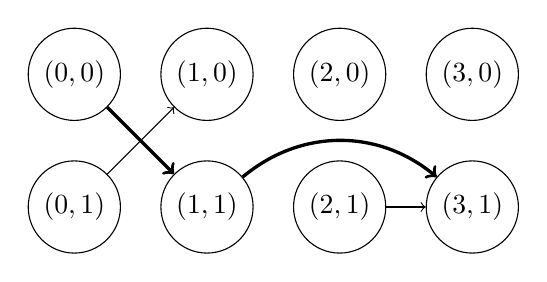
\begin{tikzpicture}[->,auto,node distance=0.5cm]
       \node[state] (q_0)                      {$(0, 0)$};
       \node[state] (q_1) [right=of q_0] {$(1, 0)$};
       \node[state] (q_2)  [right=of q_1] {$(2, 0)$};
       \node[state] (q_3) [right=of q_2] {$(3, 0)$};
       \node[state] (q_4)  [below=of q_0] {$(0, 1)$};
       \node[state] (q_5)  [right=of q_4] {$(1, 1)$};
      \node[state] (q_6)  [right=of q_5] {$(2, 1)$};
       \node[state] (q_7)  [right=of q_6] {$(3, 1)$};
       \path[->]
        (q_0) edge[very thick]  node {} (q_5)
        (q_4) edge  node {} (q_1)
        (q_5) edge [bend left, out=40, in=140, below, very thick]  node {} (q_7)
        (q_6) edge   node {} (q_7)
        ;
    \end{tikzpicture}
    \caption{The Kronecker product graph of RSM $R$ and the input graph $\mathcal{G}$ (edges which form new paths are thick)}
    \label{fig:example_1_product}
\end{figure}

This path starts in the vertex $(0,0)$ and finishes in the vertex $(3,1)$.
We can see, that 0 and 3 are the start and final states of some component
state machine for label $S$ in $R$ respectively. Thus we can conclude that
there exists a path between vertices 0 and 1 in the graph, such that the
respective word is derivable from $S$ in the $R$ execution flow.

As a result, we can add the edge $(0,S,1)$ to the resulting graph, what is done by updating the matrix $M_2^S$.

\textbf{The second iteration.} The modified graph Boolean adjacency matrices contain
an edge with label $S$. Therefore, this label contributes to the non-empty
corresponding matrix block in the evaluated matrix $M_{3,{2}}$. The transitive closure
evaluation introduces three new paths $(0, 1) \rightarrow (2,1), (1, 0) \rightarrow (3,1)$ and $(0, 1) \rightarrow (3,1)$ (see Figure~\ref{fig:example_2_product}). Since only the path between vertices $(0,1)$ and
$(3,1)$ connects the start and final states in the automaton, the edge $(1,S,1)$ is added to the resulting graph.
{
    \renewcommand{\arraystretch}{0.5}
    \setlength\arraycolsep{0.1pt}
\begin{align*}
  \centering
& M_{3,(2)} = M_1^a \otimes M_{2,(2)}^a +  M_1^b \otimes M_{2,(2)}^b + M_1^S \otimes M_{2,(2)}^S = \\
& \kbordermatrix{
          & (0,0) & (0,1) & \vrule & (1,0) & (1,1) & \vrule &  (2,0) & (2,1) & \vrule &  (3,0) & (3,1) &\\
    (0,0) & . & .  & \vrule & . & 1  & \vrule & . & .  &  \vrule & . & .  \\
    (0,1) & . & .  & \vrule & 1 & .   & \vrule & . & .  &  \vrule & . & .  \\
    \hline
    (1,0) & . & .   & \vrule & . & .  & \vrule & . & \mc  & \vrule & . & . \\
    (1,1) & . & .   & \vrule & . & .  & \vrule & . & .  & \vrule & .  &1   \\
    \hline
    (2,0) & . & .   & \vrule & . & .  & \vrule & . & .  & \vrule & . & .  \\
    (2,1) & . & .   & \vrule & . & .  & \vrule & . & .  & \vrule & . &1  \\
    \hline
    (3,0) & . & .   & \vrule & . & .  & \vrule & . & .  & \vrule & . & .  \\
    (3,1) & . & .   & \vrule & . & .  & \vrule & . & .  & \vrule & . & .  \\
}
\end{align*}
}
\begin{figure}[h]
    \centering
   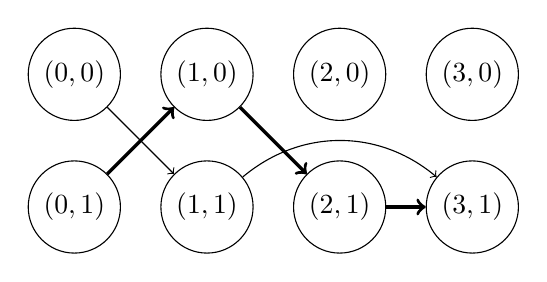
\begin{tikzpicture}[->,auto,node distance=0.5cm]
       \node[state] (q_0)                      {$(0, 0)$};
       \node[state] (q_1) [right=of q_0] {$(1, 0)$};
       \node[state] (q_2)  [right=of q_1] {$(2, 0)$};
       \node[state] (q_3) [right=of q_2] {$(3, 0)$};
       \node[state] (q_4)  [below=of q_0] {$(0, 1)$};
       \node[state] (q_5)  [right=of q_4] {$(1, 1)$};
      \node[state] (q_6)  [right=of q_5] {$(2, 1)$};
       \node[state] (q_7)  [right=of q_6] {$(3, 1)$};
       \path[->]
        (q_1) edge[very thick] node {} (q_6)
        (q_0) edge node {} (q_5)
        (q_4) edge[very thick]  node {} (q_1)
        (q_5) edge [bend left, in=140, out=40, below]  node {} (q_7)
        (q_6) edge[very thick]   node {} (q_7)
        ;
    \end{tikzpicture}
    \caption{The Kronecker product graph of RSM $R$ and the updated graph $\mathcal{G}$ (edges which form new paths are thick)}
    \label{fig:example_2_product}
\end{figure}
The result graph is presented in Figure~\ref{fig:example_result}.
\begin{figure}[h]
    \centering
    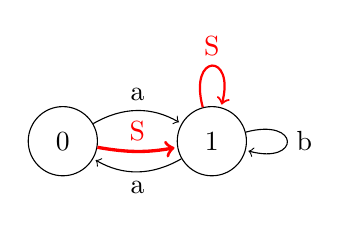
\begin{tikzpicture}[shorten >=1pt,auto]
       \node[state] (q_0)                      {$0$};
       \node[state] (q_1) [right=of q_0]       {$1$};
        \path[->]
        (q_0) edge[bend left, above]   node {a} (q_1)
         (q_0) edge[in=190, out=-10, red, very thick]   node {S} (q_1)
        (q_1) edge [bend left, below] node {a} (q_0)
         (q_1) edge[loop above, red, thick] node {S} (q_1)
        (q_1) edge[loop right] node {b} (q_1);

    \end{tikzpicture}
    \caption{The result graph $\mathcal{G}$}
    \label{fig:example_result}
\end{figure}


\begin{figure}[h]
	\centering
	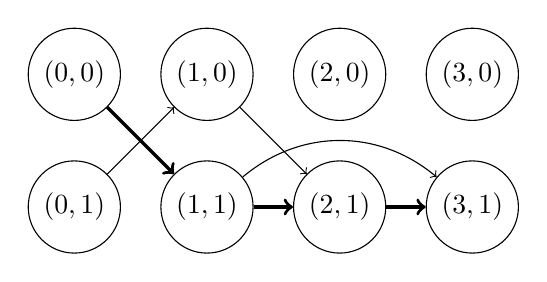
\begin{tikzpicture}[->,auto,node distance=0.5cm]
		\node[state] (q_0)                      {$(0, 0)$};
		\node[state] (q_1) [right=of q_0] {$(1, 0)$};
		\node[state] (q_2)  [right=of q_1] {$(2, 0)$};
		\node[state] (q_3) [right=of q_2] {$(3, 0)$};
		\node[state] (q_4)  [below=of q_0] {$(0, 1)$};
		\node[state] (q_5)  [right=of q_4] {$(1, 1)$};
		\node[state] (q_6)  [right=of q_5] {$(2, 1)$};
		\node[state] (q_7)  [right=of q_6] {$(3, 1)$};
		\path[->]
		(q_1) edge node {} (q_6)
		(q_0) edge[very thick] node {} (q_5)
		(q_4) edge  node {} (q_1)
		(q_5) edge [bend left, in=140, out=40, below]  node {} (q_7)
		(q_5) edge[very thick]   node {} (q_6)
		(q_6) edge[very thick]   node {} (q_7)
		;
	\end{tikzpicture}
	\caption{The Kronecker product graph of RSM $R$ and the final graph $\mathcal{G}$ (edges which form new paths are thick)}
	\label{fig:example_3_product}
\end{figure}


No more edges will be added to the graph $\mathcal{G}$ at the last iteration.
However, the new edge $(1, 1) \rightarrow (2,1)$ will be added to the resulting Kronecker product, and the transitive closure
evaluation introduces one new path $(0, 0) \rightarrow (3,1)$ that connects the start and final states in the automaton (see Figure~\ref{fig:example_3_product}).
At this point, the index creation is finished.
One can use it to answer reachability queries, but it also can be used
to restore paths for some reachable vertices. The resulting Kronecker product matrix
$M_3$, or so-called \textit{index}, can be used for it.
For example, we can restore paths from vertex 1 to vertex 1 derived from $S$ in the resulting graph.

To get these paths we should call \verb|getPaths(1, 1, S)| function.
A partial trace of this call is presented in Figure~\ref{trc:example}.
First, we query paths for all possible start and final states of the
machine for the provided graph vertices.
Since the component state machine with label $S$ in the example RSM has the single final state, the function \verb|genPaths| is called with the arguments $(0,1)$ and $(3,1)$.
Note, that the values passed to the functions in the path extraction algorithm are the
pairs of the machine state and graph vertex, which uniquely identify a cell of
the index matrix $M_3$. As a result,
we get the set of all possible paths in the graph from $1$ to $1$ derived from $S$.

\begin{figure}
\begin{minipage}[t]{0.48\textwidth}
{
\scriptsize
\setlength{\DTbaselineskip}{8pt}
\DTsetlength{0.2em}{0.5em}{0.2em}{0.4pt}{1.6pt}
\dirtree{%
.1 getPaths($1,1,S$).
.2 genPaths($(0,1),(3,1)$).
.3 return $\{[((0,1),(1,0)), ((1,0),(2,1)), ((2,1),(3,1))]\}$.
.2 currentSubPaths = $\{[1 \xrightarrow{a} 0]\}$.
.2 currentPaths = $\{[(1 \xrightarrow{a} 0)]\}$.
.2 getPaths($0,1,S$).
.3 genPaths($(0,0),(3,1)$).
.4 return $\{[((0,0),(1,1)), ((1,1),(3,1))], [((0,0),(1,1)), ((1,1),(2,1)), ((2,1),(3,1))]\}$.
.3 path = $[((0,0),(1,1)), ((1,1),(3,1))]$.
.3 currentSubPaths = $\{[0 \xrightarrow{a} 1]\}$.
.3 currentPaths = $\{[0 \xrightarrow{a} 1]\}$.
.3 currentSubPaths = $\{[1 \xrightarrow{b} 1]\}$.
.3 $\cdots$.
.3 resultPaths = $\{[0 \xrightarrow{a} 1 \xrightarrow{b} 1]\}$.
.3 path = $[((0,0),(1,1)), ((1,1),(2,1)), ((2,1),(3,1))]$.
.3 currentSubPaths = $\{[0 \xrightarrow{a} 1]\}$.
.3 currentPaths = $\{[0 \xrightarrow{a} 1]\}$.
.3 getPaths(1, 1, S) // \begin{minipage}[t]{14cm} An alternative way to get paths from 1 to 1 (leads to infinite set of paths) \end{minipage}.
.3 $\cdots$.
.8 return $r_\infty^{1 \leadsto 1}$ // \begin{minipage}[t]{5cm} An infinite set of path from 1 to 1 \end{minipage}.
.3 currentPaths = $\{[0 \xrightarrow{a} 1] \} \cdot r_\infty^{1\leadsto 1}$.
.3 currentSubPaths = $\{[1 \xrightarrow{b} 1]\}$.
.3 $\cdots$.
.3 return $\{[0 \xrightarrow{a} 1 \xrightarrow{b} 1]\} \cup (\{[0 \xrightarrow{a} 1] \} \cdot r_\infty^{1\leadsto 1} \cdot \{[1 \xrightarrow{b} 1]\})$.
.2 currentPaths = $\{[1 \xrightarrow{a} 0 \xrightarrow{a} 1 \xrightarrow{b} 1]\} \cup (\{[1 \xrightarrow{a} 0 \xrightarrow{a} 1] \} \cdot r_\infty^{1\leadsto 1} \cdot \{[1 \xrightarrow{b} 1]\})$.
.2 currentSubPaths = $\{[1 \xrightarrow{b} 1]\}$.
.2 $\cdots$.
.2 return = $\{[1 \xrightarrow{a} 0 \xrightarrow{a} 1 \xrightarrow{b} 1 \xrightarrow{b} 1]\} \cup (\{[1 \xrightarrow{a} 0 \xrightarrow{a} 1] \} \cdot r_\infty^{1\leadsto 1} \cdot \{[1 \xrightarrow{b} 1 \xrightarrow{b} 1]\})$.
}
}
\caption{Example of call stack trace}
\label{trc:example}
\end{minipage}
\end{figure}
\section{Evaluation}

The goal of this evaluation is to investigate the applicability of the proposed algorithm to both regular and context-free path querying.
We measured the execution time of the index creation which solves the reachability problem for both kinds of queries.
The execution time for CFPQ was compared with the Azimov's algorithm for CFPQ reachability.
We also investigated the practical applicability of paths extraction algorithm to both regular and context-free path queries.

For evaluation, we used a PC with Ubuntu 18.04 installed.
It has Intel core i7-6700 CPU, 3.4GHz, and DDR4 64Gb RAM.
We only measure the execution time of the algorithms themselves, thus we assume an input graph is loaded into RAM in the form of its adjacency matrix in the sparse format.
Note, that the time needed to load an input graph into the RAM is excluded from the time measurements.

\subsection{RPQ Evaluation}

To investigate the applicability of the proposed algorithm for regular path querying we gathered a dataset which consists of both real-world and synthetically generated graphs.
We generated the queries from the most popular RPQ templates.

\subsubsection{Dataset}

We gathered several graphs which represent real-world data from different areas and are frequently used for evaluation of the graph querying algorithms.
Namely, the dataset consists of three parts.
The first part is the set of LUBM graphs\footnote{Lehigh University Benchmark (LUBM) web page: \url{http://swat.cse.lehigh.edu/projects/lubm/}. Access date: 07.07.2020.}~\citep{10.1016/j.websem.2005.06.005} which have different numbers of vertices.
The second one is the set of graphs from Uniprot database\footnote{Universal Protein Resource (UniProt) web page: \url{https://www.uniprot.org/}. All files used can be downloaded via the link: \url{ftp://ftp.uniprot.org/pub/databases/uniprot/current_release/rdf/}. Access date: 07.07.2020.}: \textit{proteomes}, \textit{taxonomy} and \textit{uniprotkb}.
The~last part consists of the RDF files \textit{mappingbased\_properties} from DBpedia\footnote{DBpedia project web site: \url{https://wiki.dbpedia.org/}. Access date: 07.07.2020.} and \textit{geospecies}\footnote{The Geospecies RDF: \url{https://old.datahub.io/dataset/geospecies}. Access date: 07.07.2020.}.
A brief description of the graphs in the dataset is presented in Table~\ref{tbl:graphs_for_rpq}.

\begin{table}
    \centering
\caption{Graphs for RPQ evaluation}
\label{tbl:graphs_for_rpq}
{

\rowcolors{2}{black!2}{black!10}
\begin{tabular}{|l|c|c|}
\hline
Graph & \#V & \#E  \\
\hline
\hline
LUBM1k  & 120 926 & 484 646 \\
LUBM3.5k  & 358 434 & 144 9711 \\
LUBM5.9k  & 596 760 & 2 416 513 \\
LUBM1M   & 1 188 340 & 4 820 728 \\
LUBM1.7M & 1 780 956 & 7 228 358 \\
LUBM2.3M & 2 308 385 & 9 369 511 \\
\hline
Uniprotkb & 6 442 630 & 24 465 430 \\
Proteomes & 4 834 262 & 12 366 973 \\
Taxonomy & 5 728 398 & 14 922 125 \\
\hline
Geospecies & 450 609 & 2 201 532 \\
Mappingbased\_properties & 8 332 233 & 25 346 359 \\
\hline
\end{tabular}
}
\end{table}


Queries for evaluation were generated from the templates for the most popular RPQs, specifically the queries presented in Table 2 in~\cite{Pacaci2020RegularPQ} and in Table 5 in~\cite{Wang2019}.
These query templates are presented in Table~\ref{tbl:queries_templates}.
We generate 10 queries for each template and each graph.
The most frequent relations from the given graph were used as symbols in the query template\footnote{Used generator is available as part of CFPQ\_data project: \url{https://github.com/JetBrains-Research/CFPQ_Data/blob/master/tools/gen_RPQ/gen.py}. Access data: 07.07.2020.}.
We used the same set of queries for all LUBM graphs to investigate scalability of the proposed algorithm.

\begin{table}
    \centering
\caption{Queries templates for RPQ evaluation}
\label{tbl:queries_templates}
{\small
\renewcommand{\arraystretch}{1.2}
\rowcolors{2}{black!2}{black!10}
\begin{tabular}{|c|c||c|c|}
\hline

Name & Query & Name & Query \\
\hline
\hline
$Q_1$   & $a^*$                               & $Q_9^5$    & $(a \mid b \mid c \mid d \mid e)^+$                     \\
$Q_2$   & $a\cdot b^*$                        & $Q_{10}^2$ & $(a \mid b) \cdot c^*$                                  \\
$Q_3$   & $a \cdot b^* \cdot c^*$             & $Q_{10}^3$ & $(a \mid b \mid c)  \cdot d^*$                          \\
$Q_4^2$ & $(a \mid b)^*$                      & $Q_{10}^4$ & $(a \mid b \mid c \mid d)  \cdot e^*$                   \\
$Q_4^3$ & $(a \mid b \mid c)^*$               & $Q_{10}^5$ & $(a \mid b \mid c \mid d \mid e)  \cdot f^*$            \\
$Q_4^4$ & $(a \mid b \mid c \mid d)^*$        & $Q_{10}^2$ & $a \cdot b$                                             \\
$Q_4^5$ & $(a \mid b \mid c \mid d \mid e)^*$ & $Q_{11}^3$ & $a \cdot b \cdot c$                                     \\
$Q_5$   & $a \cdot b^* \cdot c$               & $Q_{11}^4$ & $a \cdot b \cdot c \cdot d$                             \\
$Q_6$   & $a^* \cdot b^*$                     & $Q_{11}^5$ & $a \cdot b \cdot c \cdot d \cdot f$                     \\
$Q_7$   & $a \cdot b \cdot c^*$               & $Q_{12}$   & $(a \cdot b)^+ \mid  (c \cdot d)^+$                     \\
$Q_8$   & $a? \cdot b^*$                      & $Q_{13}$   & $(a \cdot(b \cdot c)^*)^+ \mid  (d \cdot f)^+$          \\
$Q_9^2$ & $(a \mid b)^+$                      & $Q_{14}$   & $(a \cdot b \cdot (c \cdot d)^*)^+  \cdot (e \mid f)^*$ \\
$Q_9^3$ & $(a \mid b \mid c)^+$               & $Q_{15}$   & $(a \mid b)^+ \cdot (c \mid d)^+$                       \\
$Q_9^4$ & $(a \mid b \mid c \mid d)^+$        & $Q_{16}$   & $a \cdot b \cdot (c \mid d \mid e)$                     \\
\hline
\end{tabular}
}
\end{table}


\subsubsection{Results}

We averaged the execution time of index creation over 5 runs for each query.
Index creation time for LUBM graphs set is presented in Figure~\ref{fig:lubm_all_qs}.
We can see that evaluation time depends on the query: there are queries which evaluate in less than 1 second even for the largest graphs ($Q_2$, $Q_5$, $Q_{11}^2$, $Q_{11}^3$), while the worst time is 6.26 seconds ($Q_{14}$).
The execution time of our algorithm is comparable with the recent results for the same graphs and queries implemented on a distributed system over 10 nodes~\citep{Wang2019}, while we use only one node.
We conclude that our algorithm demonstrates reasonable performance to be applied to the real-world data analysis.
%\cho{Note that the accurate comparison of different approaches may be a promising direction of future research.}

\begin{figure}
    \centering
   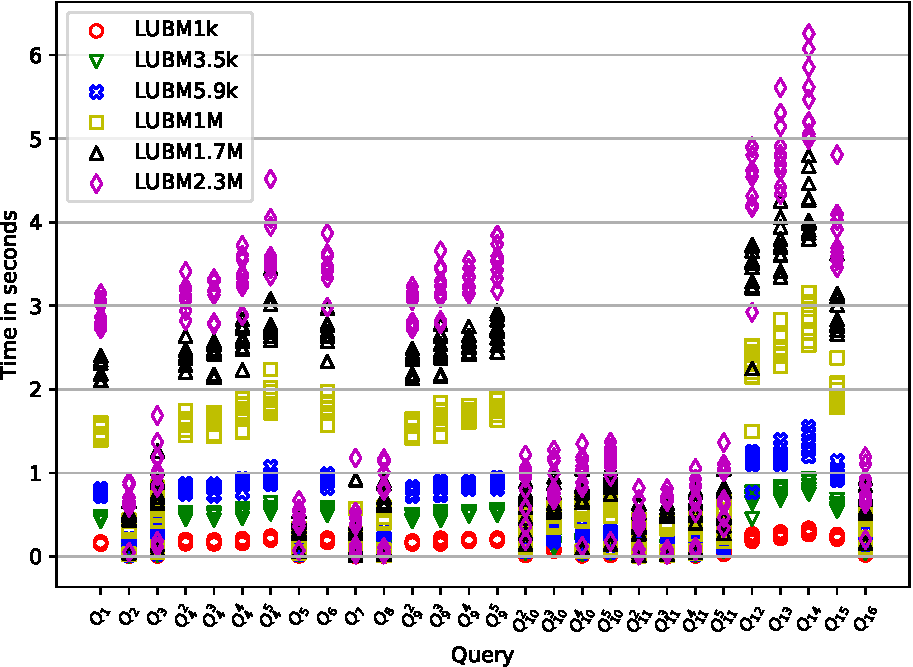
\includegraphics[width=0.6\textwidth]{data/LUBM_all.pdf}
   \caption{Index creation time for LUBM graphs}
   \label{fig:lubm_all_qs}
\end{figure}

Index creation time for each query on the real-world graphs is presented in Figure~\ref{fig:other_all_qs}.
We can see that querying small graphs requires more time than querying bigger graphs in some cases.
For example, conseder $Q_{10}^4$: querying the \textit{geospecies} graph (450k vertices) in some cases requires more time than querying of \textit{mappingbased\_properties} (8.3M vertices) and \textit{taxonomy} (5.7M vertices).
We conclude that the evaluation time depends on the inner structure of a graph.
On the other hand, \textit{taxonomy} querying in many cases requires significantly more time than for other graphs, while \textit{taxonomy} is not the biggest graph.
Finally, in most cases query execution lasts less than 10 seconds, even for bigger graphs, and no query requires more than 52.17 seconds.

\begin{figure}
    \centering
   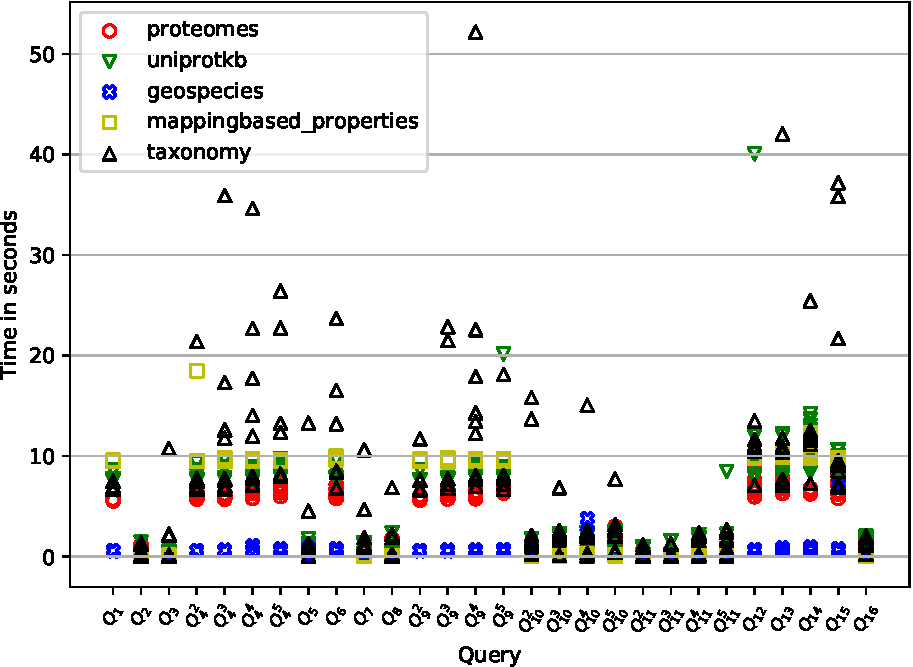
\includegraphics[width=0.6\textwidth]{data/other_all.pdf}
   \caption{Index creation time for real-world RDFs}
   \label{fig:other_all_qs}
\end{figure}

%We evaluate path extraction for queries which result in possibly long paths.
%Long paths usually require many iterations of transitive closure evaluation, thus we used the number of the iterations as a criterion to select the inputs for the evaluation.
%For each selected graph and query we measure paths extraction time for each reachable pair.
%Since the index can be reused from the previous step, we omit the time necessary to create the index.
%We limit by 10 the number of paths to extract.

%In Figures~\ref{fig:geo_tensors_rpq} and~\ref{fig:dbpedia_tensors_rpq} we show the time needed to extract a path of a specific length when only one path was extracted.
%The main observation is that time is linear on the path length, even if a generic path extraction procedure is used.

%\begin{figure}
%     \begin{subfigure}[b]{0.45\textwidth}
%         \centering
%         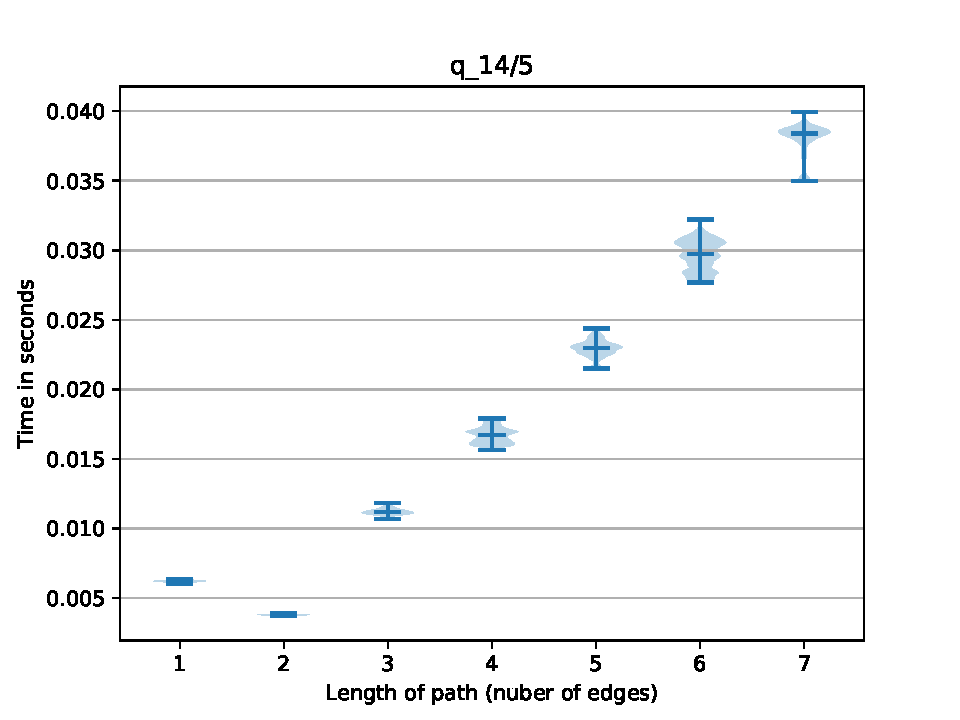
\includegraphics[width=\textwidth]{../paper/data/geo_rpq_single_path/q_14_5.pdf}
%         \caption{\footnotesize \textit{geospecies}, $Q_{14}$}
%         \label{fig:geo_tensors_rpq}
%     \end{subfigure}
%     ~\begin{subfigure}[b]{0.45\textwidth}
%         \centering
%         \includegraphics[width=\textwidth]{../paper/data/CF/Tensor_path/dbpedia_path_tensor.pdf}
%         \caption{\footnotesize \textit{mappingbased\_properties}, $Q_{4}^5$}
%         \label{fig:dbpedia_tensors_rpq}
%     \end{subfigure}\\
%     \begin{subfigure}[b]{0.45\textwidth}
%         \centering
%         \includegraphics[width=\textwidth]{../paper/data/CF/Matrix_CF/geo_path_matrix.pdf}
%         \caption{\footnotesize \textit{geospecies}, \textit{Geo}}
%         \label{fig:geo_matrix_cfpq}
%     \end{subfigure}
%     ~\begin{subfigure}[b]{0.45\textwidth}
%         \centering
%         \includegraphics[width=\textwidth]{../paper/data/CF/Tensor_path/geo_path_tensor.pdf}
%         \caption{\footnotesize \textit{geospecies}, \textit{Geo}}
%         \label{fig:geo_tensors_cfpq}
%     \end{subfigure}\\
%   \caption{Single path extraction for specific graph and query for our solution (\subref{fig:geo_tensors_rpq}, \%subref{fig:dbpedia_tensors_rpq}, \subref{fig:geo_tensors_cfpq}), and Azimov's (\subref{fig:geo_matrix_cfpq})}
%\end{figure}

\subsection{CFPQ Evaluation}

We evaluate the applicability of the proposed algorithm to CFPQ processing over real-world graphs on a number of classic cases and compare them with the Azimov's algorithm.
Currently only a single path version of Azimov's algorithm exists, and we use its implementation using PyGraphBLAS. Note that it is not trivial to compare our results with the state-of-the-art results provided by~\cite{10.1145/3398682.3399163} (Azimov's algorithm) because our algorithm computes significantly more information. While the state-of-the-art solution computes only reachability facts or a single-path semantics, our algorithm computes data necessary to restore all possible paths.

\subsubsection{Dataset}

We use CFPQ\_Data\footnote{CFPQ\_Data is a dataset for CFPQ evaluation which contains both synthetic and real-world data and queries \url{https://github.com/JetBrains-Research/CFPQ\_Data}. Access date: 07.07.2020.} dataset for evaluation.
Namely, we use relatively big RDF files and respective same-generation queries $G_1$~(Eq.~\ref{eqn:g_1}) and $G_2$~(Eq.~\ref{eqn:g_2}) which are used in other works for CFPQ evaluation.
We also use the $Geo$~(Eq.~\ref{eqn:geo}) query provided by~\cite{Kuijpers:2019:ESC:3335783.3335791} for \textit{geospecies} RDF.
Note that we use $\overline{x}$ notation in queries to denote the inverse of $x$ relation and the respective edge.
\begin{align}
\begin{split}
\label{eqn:g_1}
S \to & \overline{\textit{subClassOf}} \ \ S \ \textit{subClasOf} \mid \overline{\textit{type}} \ \ S \ \textit{type}\\   & \mid \overline{\textit{subClassOf}} \ \ \textit{subClasOf} \mid \overline{\textit{type}} \ \textit{type}
\end{split}
\end{align}
\begin{align}
\begin{split}
\label{eqn:g_2}
S \to \overline{\textit{subClassOf}} \ \ S \ \textit{subClasOf} \mid \textit{subClassOf}
\end{split}
\end{align}
\begin{align}
\begin{split}
\label{eqn:geo}
S \to & \textit{broaderTransitive} \ \  S \ \overline{\textit{broaderTransitive}} \\
      & \mid \textit{broaderTransitive} \ \  \overline{\textit{broaderTransitive}}
\end{split}
\end{align}
\begin{align}
\begin{split}
\label{eqn:ma}
S & \to \overline{d} \ V \ d \\
V & \to ((S?) \overline{a})^* (S?) (a (S?))^*
\end{split}
\end{align}

Additionally we evaluate our algorithm on memory aliases analysis problem: a well-known problem which can be reduced to CFPQ~\citep{Zheng:2008:DAA:1328897.1328464}.
To do it, we use some graphs built for different parts of Linux OS kernel (\textit{arch}, \textit{crypto}, \textit{drivers}, \textit{fs}) and the query $MA$~(Eq.~\ref{eqn:ma})~\citep{10.1145/3093336.3037744}.
The detailed data about all the graphs used is presented in Table~\ref{tbl:graphs_for_cfpq}.

{\setlength{\tabcolsep}{0.3em}
\begin{table}
    \centering
{
\caption{Graphs for CFPQ evaluation: \textit{bt} is broaderTransitive, \textit{sco} is subCalssOf}
\label{tbl:graphs_for_cfpq}
\scriptsize
\rowcolors{2}{black!2}{black!10}
\begin{tabular}{|l|c|c|c|c|c|c|c|}
\hline
Graph          & \#V       & \#E        & \#sco & \#type &\#bt & \#a  & \#d \\
\hline
\hline
eclass\_514en  & 239 111    & 523 727    & 90 512    & 72 517    &        ---        & ---  & --- \\
enzyme         & 48 815     & 109 695    & 8 163     & 14 989    &        ---        & ---  & --- \\
geospecies     & 450 609    & 2 201 532  & 0         & 89 062    &        20 867     & ---  & --- \\
go             & 272 770    & 534 311    & 90 512    & 58 483    &        ---        & ---  & --- \\
go-hierarchy   & 45 007     & 980 218    & 490 109   & 0         &        ---        & ---  & --- \\
taxonomy       & 5 728 398  & 14 922 125 & 2 112 637 & 2 508 635 &        ---        & ---  & --- \\
\hline
arch           & 3 448 422  & 5 940 484  &      ---     &  ---   &        ---        & 671 295 & 2 298 947 \\
crypto         & 3 464 970  & 5 976 774  &      ---     &  ---   &        ---        & 678 408 & 2 309 979 \\
drivers        & 4 273 803  & 7 415 538  &      ---     &  ---   &        ---        & 858 568 & 2 849 201 \\
fs             & 4 177 416  & 7 218 746  &      ---     &  ---   &        ---        & 824 430 & 2 784 943 \\
\hline
\end{tabular}
}
\end{table}
}
\subsubsection{Results}

We averaged the index creation time over 5 runs for both single-path Azimov's algorithm (\textbf{Mtx}) and the proposed algorithm (\textbf{Tns}) (see Table~\ref{tbl:CFPQ_index}).

{\setlength{\tabcolsep}{0.2em}
  \begin{table}
    \centering
    \caption{CFPQ evaluation results, time is measured in seconds}
    \label{tbl:CFPQ_index}
    \rowcolors{4}{black!2}{black!10}
    \small
    \begin{tabular}{| l | c | c | c | c | c | c | c | c |}
      \hline

      \multirow{2}{*}{Name}  & \multicolumn{2}{c|}{$G_1$} & \multicolumn{2}{c|}{$G_2$} & \multicolumn{2}{c|}{\textit{Geo}} & \multicolumn{2}{c|}{\textit{MA}}\\
      \cline{2-9}
                      & Tns    & Mtx    & Tns  & Mtx  & Tns   & Mtx   & Tns     & Mtx \\
      \hline
      \hline
      eclass\_514en   & 0.24   & 0.27   & 0.25 & 0.26 & ---   & ---   & ---     & ---\\
      enzyme          & 0.03   & 0.04   & 0.02 & 0.01 & ---   & ---   & ---     & ---\\
      geospecies      & 0.08   & 0.06   & $0^{*}$ & 0.01 & 26.12 & 16.58 & ---     & ---\\
      go-hierarchy    & 0.16   & 1.43   & 0.23 & 0.86 & ---   & ---   & ---     & ---\\
      go              & 1.56   & 1.74   & 1.21 & 1.14 & ---   & ---   & ---     & ---\\
      pathways        & 0.01   & 0.01   & 0.01 & 0.01 & ---   & ---   & ---     & ---\\
      taxonomy        & 4.81   & 2.71   & 3.75 & 1.56 & ---   & ---   & ---     & ---\\
      \hline
      arch            & ---    & ---    & ---  & ---  & ---   & ---   & 262.45  & 195.51  \\
      crypto          & ---    & ---    & ---  & ---  & ---   & ---   & 267.52  & 195.54  \\
      drivers         & ---    & ---    & ---  & ---  & ---   & ---   & 1309.57 & 1050.78 \\
      fs              & ---    & ---    & ---  & ---  & ---   & ---   & 470.49  & 370.73  \\
      \hline
    \end{tabular}
  \end{table}
}

Best to our knowledge, the proposed algorithm is the first algorithm that provides information about all paths of interest (Azimov's algorithm computes information about only one path).
The direct comparison with other solutions is impossible, and we just estimate the running time of our algorithm for a small number of cases.
Namely, we extract all paths with length not greater than 20 edges between all pairs of vertices from indeces created for graphs \textit{go} and \textit{eclass\_514en} and query $G_1$.
Paths extraction for one pair of vertices requires 2.64 seconds averaged over all pairs for \textit{go} graph. The~maximal time is 4699 seconds and 217737 paths were extracted during this time. The average number of paths between two vertices is 184.
For \textit{eclass\_514en} paths extraction for one pair of vertices requires 1.27 seconds averaged over all pairs. The~maximal time is 8.04 seconds and only one path is extracted during this time. The average number of paths between two vertices is 3.
We can see that paths can be extracted in a reasonable time, but a detailed analysis of paths extraction algorithm performance depends on graphs structure.

%Comparison of paths extraction is presented in Figures~\ref{fig:geo_matrix_cfpq} and~\ref{fig:geo_tensors_cfpq}.
%While both methods demonstrate linear time on the length of the extracted path, our generic solution is more than 1000 times slower than Azimov's single path extraction procedure.
%We conclude that current generic all-path extraction procedure is not optimal for single path extraction.

\subsection{Conclusion}

We conclude that the proposed algorithm is applicable to real-world data processing: the algorithm allows one to solve both the reachability problem and to extract paths of interest in a reasonable time even using naive implementation.
While index creation time (reachability query evaluation) is comparable with other existing solutions, paths extraction procedure should be improved in the future. However, the state-of-the-art solution computes only reachability facts or a single-path semantics, whereas our algorithm computes data necessary to restore all possible paths (all-paths semantics).
Finally, a detailed comparison of the proposed solution with other algorithms for CFPQ and RPQ is required.

To summarize the overall evaluation, the proposed algorithm is applicable to both RPQ and CFPQ over real-world graphs.
Thus, the proposed solution is a promising unified algorithm for both RPQ and CFPQ evaluation.

\section{Related Work}

Language constrained path querying is widely used in graph databases, static code analysis, and other areas.
Both, RPQ and CFPQ (known as CFL reachability problem in static code analysis) are actively studied in the recent years.

There is a huge number of theoretical research on RPQ and its specific cases.
RPQ with single-path semantics was investigated from the theoretical point of view by~\cite{barrett2000formal}.
In order to research practical limits and restrictions of RPQ, a number of high-performance RPQ algorithms were provided.
For example, the derivative-based solution provided by~\cite{10.1145/2949689.2949711}, which is implemented on top of the Pregel-based system, or the solution by~\cite{10.1007/978-3-642-31235-9_12}.
But only a limited number of practical solutions provide the ability to restore paths of interest.
A recent work by~\cite{Wang2019} provides a Pregel-based provenance-aware RPQ algorithm which utilizes a Glushkov's construction~\citep{Glushkov1961}.
There is a lack of research of the applicability of linear algebra-based RPQ algorithms with paths-providing semantics.

On the other hand, many CFPQ algorithms with various properties were proposed recently.
They employ the ideas of different parsing algorithms, such as CYK in works by~\cite{hellingsRelational} and~\cite{8249039}, (G)LR and (G)LL in works by~\cite{10.1007/978-3-319-41579-6_22},~\cite{Grigorev:2017:CPQ:3166094.3166104},~\cite{10.1007/978-3-319-91662-0_17},~\cite{Medeiros:2018:EEC:3167132.3167265}.
Unfortunately, none of them has better than cubic time complexity in terms of the input graph size.
The algorithm by~\cite{Azimov:2018:CPQ:3210259.3210264} is, best to our knowledge, the first algorithm for CFPQ which is based on linear algebra.
It was shown by~\cite{10.1145/3398682.3399163} that this algorithm can be applied to real-world graph analysis problems, while~\cite{Kuijpers:2019:ESC:3335783.3335791} show that other state-of-the-art CFPQ algorithms are not performant enough to handle real-world graphs.

It is important in both RPQ and CFPQ to be able to restore paths of interest.
Some of the mentioned algorithms can solve only the reachability problem, while it may be important to provide at least one path which satisfies the query.
While~\cite{10.1145/3398682.3399163} provide the first CFPQ algorithm with single path semantics based on linear algebra,~\cite{HellSinglePath} provides the first theoretical investigation of this problem.
He also provides an overview of the related works and shows that the problem is related to the string generation problem and respective results from the formal language theory.
He concludes that both theoretical and empirical investigation of CFPQ with single-path and all-path semantics are at the early stage.
We agree with this point of view, and we only demonstrate the applicability of our solution to paths extraction and do not investigate its properties in details.

While CFPQ on $n$-node graph has a relatively straightforward $O(n^3)$ time algorithm, it is a long-standing open problem whether there exists a truly  subcubic $O(n^{3-\varepsilon})$ algorithm for this problem.
The question on the existence of a subcubic CFPQ algorithm was stated by~\cite{Yannakakis}.
A bit later~\cite{10.5555/271338.271343} proposed the CFL reachability as a framework for interprocedural static code analysis.
\cite{10.1145/258994.259006} gave a dynamic programming formulation of the problem which runs in $O(n^3)$ time.
The problem of the cubic bottleneck of context-free language reachability is also discussed by~\cite{10.5555/788019.788876} and~\cite{10.1145/258994.259006}.
The slightly subcubic algorithm with $O(n^3/\log{n})$ time complexity was provided by~\cite{10.1145/1328438.1328460}.
This result is inspired by recursive state machine reachability.
The first truly subcubic algorithm with $O(n^\omega polylog(n))$ time complexity ($\omega$ is the best exponent for matrix multiplication) for an arbitrary graph and 1-Dyck language was provided by~\cite{8249039}, and~\cite{pavlogiannis2020finegrained}.
Other partial cases were investigated by~\cite{10.1145/3158118},~\cite{zhang2020conditional}.

Employing linear algebra is a promising way to high-performance graph analysis.
There are many works which formulate specific graph algorithms in terms of linear algebra, for example, such algorithms as for computing transitive closure and all-pairs shortest paths.
Recently this direction was summarized in GrpahBLAS API~\citep{7761646} which provides building blocks to develop a graph analysis algorithm in terms of linear algebra.
There is a number of implementations of this API, such as SuiteSparse:GraphBLAS~\citep{10.1145/3322125} or CombBLAS~\citep{10.1177/1094342011403516}.
Approaches to evaluate different classes of queries in different systems based on linear algebra are being actively researched.
This approach demonstrates significant performance improvement when applied for SPARQL queries evaluation~\citep{10.1145/3302424.3303962,DBLP:journals/corr/MetzlerM15a} and for Datalog queries evaluation~\citep{sato_2017}.
Finally, RedisGraph~\citep{8778293}, a linear-algebra powered graph database, was created and it was shown that in some scenarios it outperforms many other graph databases.
\section{Conclusion}

Conclusion, current state, results.

Future work. Library extension up to full GraphBLAS API implementation.

LaGraph on F\# .NET.

Evaluation. Comparison with other implementations on different devices.
Manual implementation versus translation.  

Another direction of future work is Brahma.FSharp improvements. 
First of all, it is necessary to support discriminated unions to make it possible to express custom semirings such as \texttt{Min-Plus}, as presented in listing~\ref{lst_example}. 

Also, it is necessary to add high-level abstractions for asynchronous programming, and for multi-GPU programming.
Such mechanisms can be naturally expressed in F\# with native primitives for asynchronous programming.

fusion and other optimizations.
% Authors must disclose all relationships or interests that 
% could have direct or potential influence or impart bias on 
% the work: 
%
% \section*{Conflict of interest}
%
% The authors declare that they have no conflict of interest.


% BibTeX users please use one of
%\bibliographystyle{spbasic}      % basic style, author-year citations
%\bibliographystyle{spmpsci}      % mathematics and physical sciences
%\bibliographystyle{spphys}       % APS-like style for physics
%\bibliography{}   % name your BibTeX data base

\bibliographystyle{spbasic}  
\bibliography{tensor_product_CFPQ}
\end{document}
% end of file template.tex

